% -----------------------------------------------
% Template for JIM
%     jim.sty -> style file
% By Eloi Batlle (eloi@iua.upf.es), changes for 
% ICMC by Bram de Jong (bdejong@iua.upf.es)
% changes for JIM 2007 by Dominique Fober (fober@grame.fr)
% changes for JIM 2009 by Olivier Tache (olivier.tache@imag.fr)
% -----------------------------------------------

\documentclass{article}
\usepackage{jim,amsmath}
\usepackage[utf8]{inputenc}
\usepackage[francais]{babel}
\usepackage[T1]{fontenc}
%\usepackage{pxfonts}
\usepackage{graphicx}

\hyphenation{com-me gra-phi-que} 

% Title.
% ------
\title{Atelier INScore \\
\textmd{{\small Un environnement pour le design de partitions musicales augmentées interactives.}}
}

% Single \textsc{address}
% To use with only one author or several with the same address
% ---------------
\oneauthor
  {D. Fober, S. Letz, Y. Orlarey} {GRAME - Centre national de création musicale\\ \{fober, letz, orlarey\}@grame.fr}

% Two addresses
% --------------
%\twoauthors
%  {First author} {School \\ Department}
%  {Second author} {Company \\ Address}

% Three addresses
% --------------
%\threeauthors
%  {D. Fober} {Organisme \\ Adresse électronique}
%  {S. Letz} {Organisme \\ Adresse électronique}
%  {Y. Orlarey} {Organisme \\ Adresse électronique}

\begin{document}
%
\maketitle
%
\begin{abstract}
INScore est un afficheur de partitions musicales augmentées, interactives. INScore comprend un système de représentation de l'interprétation, vue comme un signal audio ou gestuel, ainsi qu'un système de représentation graphique des relations temporelles entre composants de la partition. Piloté par des messages OSC, INScore propose une approche originale au design de partitions musicales. L'atelier INScore permettra aux participants de se familiariser avec l'environnement de programmation. 
\end{abstract}

%\vspace{1cm}
\section{INScore}

INScore est un environnement pour le design de partitions musicales augmentées interactives. L'environnement est issu du projet Interlude qui vise à développer des interfaces gestuelles pour une exploration en temps-réel de contenus musicaux, dans le domaine du signal audio comme dans celui symbolique, de la partition. Dans ce contexte, la partition musicale augmentée représente un espace graphique mettant en relation un objet musical symbolique avec différentes représentations de son interprétation.

Ce concept de partition musicale augmentée s'articule autour de deux axes :
\begin{itemize}
\item la prise en compte d'objets arbitraires (notation musicale, images, texte, graphiques vectoriels) et leur \textit{synchronisation temporelle dans le domaine graphique},
\item la représentation du signal audio ou gestuel au sein de la partition.
\end{itemize}

Le travail sur ces deux axes a débouché sur une approche originale de la description des relations entre espaces temporels et graphiques \cite{fober:10b}, ainsi que sur un système dynamique de construction de \textit{signaux graphiques} \cite{fober:10a,Fober:10c} (figure \ref{fig:example}).

Plus récement, le système a été étendu avec des primitives d'interaction et une prise en charge plus autonome des médias composants la partition.

INScore est un projet Open Source publiquement disponible sur SourceForge\footnote{http://inscore.sf.net}. L'environnement fonctionne sur Mac OS, Linux et Windows. Il est piloté par des messages OSC \cite{wright02} et un grand nombre d'exemples d'utilisation sont fournis pour Max/MSP, Pure Data, Python ou Lisp.

\section{L'atelier}

L'atelier INScore a pour but de familiariser les participants avec l'environnement et l'interface de contrôle OSC. Il se déroulera en 2 parties:
\begin{itemize}
\item présentation générale de l'environnement
\item séance pratique de programmation.
\end{itemize}

Lors de la séance pratique, les participants pourront utliser indifféremment les environnements Max/MSP ou Pure Data. Il est conseillé d'installer la dernière version d'INScore au préalable.


\begin{figure}
\centerline{
	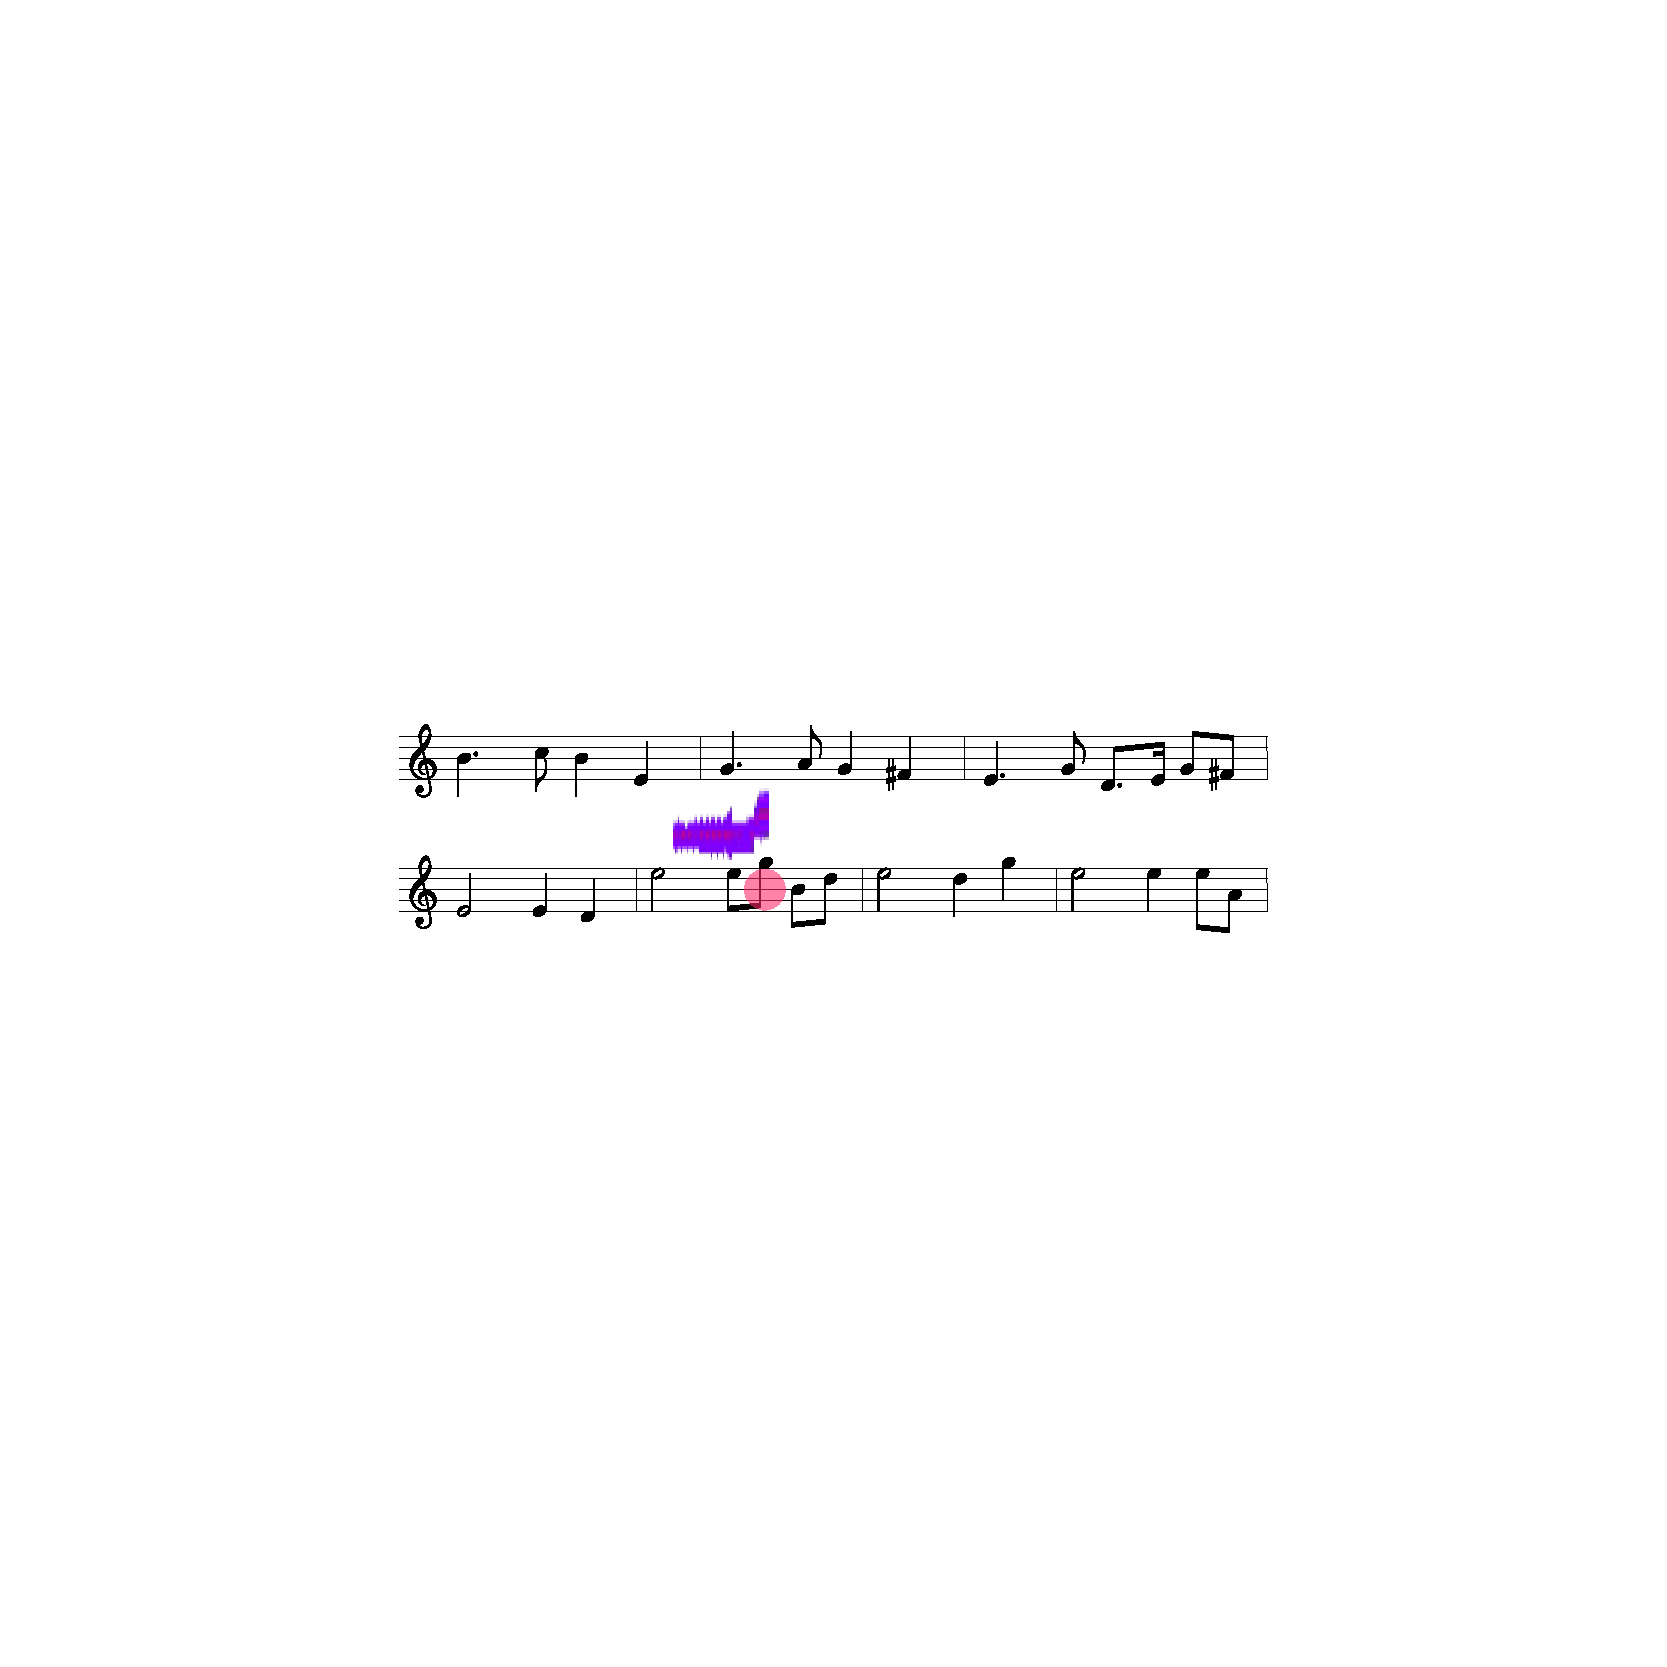
\includegraphics[width=0.95\columnwidth]{scene1}}
\caption{Un signal graphique synchronisé à une partition.}
\label{fig:example}
\end{figure}



%=============================================================
\vspace{4mm}
\hspace{-5mm}
\textbf{Remerciements} \\
INScore est issu du projet Interlude qui est soutenu par l'Agence Nationale pour la Recherche [ANR-08-CORD-010].

%\vspace{1cm}
\bibliographystyle{unsrt}
\bibliography{../interlude}

\end{document}
